\documentclass[notes]{subfiles}

\begin{document}
	\addcontentsline{toc}{section}{1.7 - The Precise Definition of a Limit}
	\refstepcounter{section}
	\fancyhead[RO,LE]{\bfseries \large\nameref{cs17}} 
	\fancyhead[LO,RE]{\bfseries \currentname}
	\fancyfoot[C]{{}}
	\fancyfoot[RO,LE]{\large \thepage}	%Footer on Right \thepage is pagenumber
	\fancyfoot[LO,RE]{\large Chapter 1.7}
	
\section*{The Precise Definition of a Limit}\label{cs17}
	\subsection*{Before Class}
	\subsubsection*{Motivating Example}
		\begin{ex}
			Let $f(x) = \begin{cases}2x + 1 & x\neq 2 \\ 1 & x = 2 \end{cases}$
			\begin{enumerate}[(a)]
				\item What is $\ds \lim_{x\to 2} f(x)$?
					\vs{.25}
				\item How close to 2 must $x$ be so that the difference between $f(x)$ and 5 is less than $0.1$?
					\vs{2}
				\item How close to 2 must $x$ be so that the difference between $f(x)$ and 5 is less than $0.001$?
					\vs{2}
					\newpage
				\item How close to 2 must $x$ be so that the difference between $f(x)$ and 5 is less than some arbitrary (small) number $\varepsilon$?
					\vs{2}
			\end{enumerate}
		\end{ex}
		
		\begin{defn}[Precise Definition of a Limit]
			Let $f$ be a function defined on some open interval that contains the number $a$ (except possibly at $a$ itself).  We say that the \textbf{limit of} $f(x)$ \textbf{as} $x$ \textbf{approaches} $a$ \textbf{is} $L$, and write
			\showto{ins}{
				\[\lim_{x\to a} f(x) = L\]
				if for every number $\varepsilon > 0$ there is a number $\delta > 0$ such that if $0 < |x-a| < \delta$, then $|f(x) - L| < \varepsilon$
			}
			\showto{st}{
			\\ \\ \\ \\ \\ \\
			}
		\end{defn}
		
		\begin{ex}
			Label the figure below using $a$, $\delta$, $L$, and $\varepsilon$ to see a graphical representation of the precise definition of the limit.
			\begin{flushleft}
				\showto{ins}{
				\begin{tikzpicture}
					\begin{axis}[
							every tick label/.append style={font=\small},
							axis x line = middle,
							axis y line = middle,
				    			every axis y label/.style={at={(ticklabel cs:1.15)}},
								y label style={at={(axis description cs: 0.2, 1)},above},
				    			ylabel = {$y$},
				    			ymin = 0, ymax = 4.5,
			    				every axis x label/.style= {at ={(ticklabel cs:1)}},
				    				x label style={at={(axis description cs: 1, 0)},right},
			    				xlabel = {$x$},
			    				xmin = -.5, xmax = 2,		
			    				xtick = {1},
			    				xticklabels = {},
			    				yticklabels = {},
			    				ytick = {3}
						]	
						
						\addplot[thick, smooth, domain = 0:1.8] {sin(deg(pi*x))+3};
							\coordinate (point) at (1,3);
							\coordinate (xlabel) at (1,-.1);
						\addplot[domain = -.1:2.] {3.75};
							\coordinate (top line) at (1.5, 3.75);
						\addplot[domain = -.1:2.] {2.25};
							\coordinate (bottom line) at (.5, 2.25);
						\addplot[densely dashed, domain = -.1:2.] {3};
							\coordinate (limit) at (2,3);
						\coordinate (top) at (0,3.7);
						\coordinate (middle1) at (0,3.05);
						\coordinate (middle2) at (0,2.95);
						\coordinate (bottom) at (0,2.3);
						
					\end{axis}
						\filldraw (point) circle (0.1);
						\draw (xlabel) node[yshift = -5pt] {$a$};
						\draw (limit) node[xshift = 15pt] {$y = L$};
						\draw (top line) node[yshift = 10pt] {$y = L + \varepsilon$};
						\draw (bottom line) node[yshift = -10pt] {$y = L - \varepsilon$};
						\draw [thick,decorate,decoration={brace,amplitude=2pt,mirror,raise=4pt},yshift=0pt] (top)--(middle1) node [black,midway, xshift = -10pt] {$\varepsilon$};
						\draw [thick,decorate,decoration={brace,amplitude=2pt,mirror,raise=4pt},yshift=0pt] (middle2)--(bottom) node [black,midway, xshift = -10pt] {$\varepsilon$};
				\end{tikzpicture}
				}
				\showto{st}{
				\begin{tikzpicture}
					\begin{axis}[
							every tick label/.append style={font=\small},
							axis x line = middle,
							axis y line = middle,
				    			every axis y label/.style={at={(ticklabel cs:1.15)}},
								y label style={at={(axis description cs: 0.2, 1)},above},
				    			ylabel = {$y$},
				    			ymin = 0, ymax = 4.5,
			    				every axis x label/.style= {at ={(ticklabel cs:1)}},
				    				x label style={at={(axis description cs: 1, 0)},right},
			    				xlabel = {$x$},
			    				xmin = -.5, xmax = 2,		
			    				xtick = {1},
			    				xticklabels = {},
			    				yticklabels = {},
			    				ytick = {3}
						]	
						
						\addplot[thick, smooth, domain = 0:1.8] {sin(deg(pi*x))+3};
							\coordinate (point) at (1,3);
							\coordinate (xlabel) at (1,-.1);
						\addplot[domain = -.1:2.] {3.75};
							\coordinate (top line) at (1.5, 3.75);
						\addplot[domain = -.1:2.] {2.25};
							\coordinate (bottom line) at (.5, 2.25);
						\addplot[densely dashed, domain = -.1:2.] {3};
							\coordinate (limit) at (2,3);
						\coordinate (top) at (0,3.7);
						\coordinate (middle1) at (0,3.05);
						\coordinate (middle2) at (0,2.95);
						\coordinate (bottom) at (0,2.3);
						
					\end{axis}
						\filldraw (point) circle (0.1);
						%\draw (xlabel) node[yshift = -5pt] {$a$};
						%\draw (limit) node[xshift = 15pt] {$y = L$};
						%\draw (top line) node[yshift = 10pt] {$y = L + \varepsilon$};
						%\draw (bottom line) node[yshift = -10pt] {$y = L - \varepsilon$};
						\draw [thick,decorate,decoration={brace,amplitude=2pt,mirror,raise=4pt},yshift=0pt] (top)--(middle1) node [black,midway, xshift = -10pt] {};
						\draw [thick,decorate,decoration={brace,amplitude=2pt,mirror,raise=4pt},yshift=0pt] (middle2)--(bottom) node [black,midway, xshift = -10pt] {};
				\end{tikzpicture}
				}
			\end{flushleft}
		\end{ex}
			\vs{.5}
			\newpage
	
	\subsubsection*{Pre-Class Activity}
		\begin{ex}
			We now have two definitions for the limit: an Intuitive Definition (see \S1.5) and a Formal Definition.  Write what \emph{you} perceive to be the similarities and differences between the two definitions.
		\end{ex}
			\vs{2}
			
		\begin{question}
			Many students are intimidated by the formal definition of a limit.  The best way to become more comfortable with it is by asking questions and clearing up ambiguities; use this space to write comments for class.
		\end{question}
			\vs{2}
	\subsubsection*{In Class}
		\begin{ex}
			Use the given graph of $f$ to find a number $\delta$ such that $|x - 1| < \delta\Rightarrow |f(x) - 1| < 0.2$.
			\begin{flushleft}
				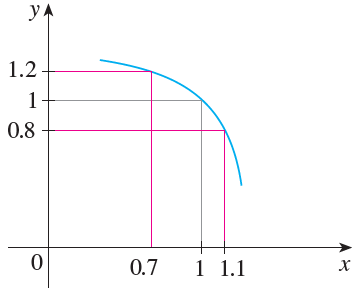
\includegraphics{1.7fig1}
			\end{flushleft}
		\end{ex}
			\newpage
			
		\begin{ex}
			Use the given graph of $f(x) = \sqrt{x}$ to find a number $\delta$ such that if $|x - 4| < \delta$, then $|f(x) - 2 | < 0.4$.	
			\begin{flushleft}
				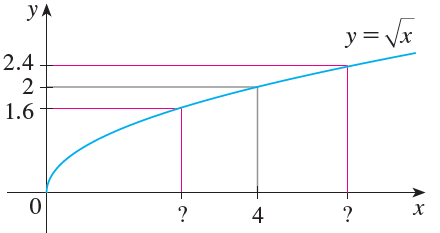
\includegraphics{1.7fig2}
			\end{flushleft}
		\end{ex}
			\vs{1}
			
		\begin{ex}
			Use the given graph of $f(x) = x^2$ to find a number $\delta$ such that if $|x - 1| < \delta$, then $|x^2 - 1| < \dfrac{1}{2}$.
			\begin{flushleft}
				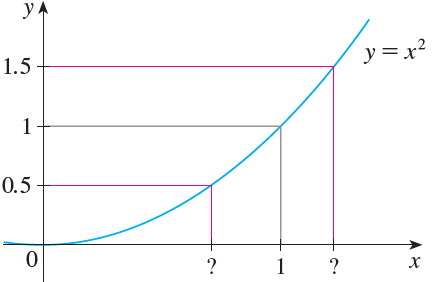
\includegraphics{1.7fig3}
			\end{flushleft}
		\end{ex}
			\vs{1}
			\newpage
			
		\begin{ex}
			Show that $\ds \lim_{x\to 6} (5x-3) = 27$
		\end{ex}
			\vs{1}
			
		\begin{ex}
			Show that $\ds \lim_{t\to 1} (2t+1) = 3$
		\end{ex}
			\vs{1}
			\newpage
			
		\begin{defn}[Formal Definition of Left/Right-Hand Limits]
			$\ds \lim_{x\to a^-} f(x) = L$ if 
			\showto{ins}{
				for every $\varepsilon > 0$, there is a number $\delta > 0$ such that if $a-\delta< x < a$, then $|f(x) - L| < \varepsilon$.  \\ \\
			}
			\showto{st}{
				\\ \\ \\
			}
			$\ds \lim_{x\to a^+} f(x) = L$ if 
			\showto{ins}{
				for every $\varepsilon > 0$, there is a number $\delta > 0$ such that if $a < x < a+\delta$, then $|f(x) - L| < \varepsilon$. 
			}
			\showto{st}{
				\\ \\ \\
			}
		\end{defn}

			
		\begin{ex}
			Use the formal definition of the limit to show that $\ds \lim_{x\to 0^+} \sqrt{x} = 0$
		\end{ex}
			\vs{1}
			\newpage
			
		\begin{ex}
			Use the formal definition of the limit to show that $\ds \lim_{x\to 2} x^2 = 4$
		\end{ex}
			\vs{1}
			\newpage
			
	\subsection*{After Class}
		\begin{ex}
			A circular gasket for a space shuttle is require to have an area of 900 square centimeters.
			\begin{enumerate}[(a)]
				\item What radius should the gasket be?
					\vs{.5}
					
				\item If the gasket is allowed to have an error tolerance of $\pm 2$ square centimeters in the area, how close to the ideal radius in part (a) must the producer control the radius? \emph{Relate this to the formal definition of the limit}.
					\vs{1}
					
				\item In terms of the $\varepsilon, \delta$ definition of the expression $\ds \lim_{x\to a} f(x) = L$, what is $x$?  What is $f(x)$?  What is $a$?  What is $L$?  What value of $\varepsilon$ is given?  What is the corresponding value of $\delta$?
					\vs{1}
			\end{enumerate}
		\end{ex}
		
		\begin{ex}
			Use the formal defintion of the limit to compute $\ds \lim_{x\to 1} (3x - 1)$.
		\end{ex}
			\vs{2}
	\clearpage
\end{document}